% \begin{savequote}[75mm]
% Nulla facilisi. In vel sem. Morbi id urna in diam dignissim feugiat. Proin molestie tortor eu velit. Aliquam erat volutpat. Nullam ultrices, diam tempus vulputate egestas, eros pede varius leo.
% \qauthor{Quoteauthor Lastname}
% \end{savequote}

\chapter{Nonlinear Interaction Networks}



Hawkes process inference relied on an augmentation strategy 
made possible by the linear form and excitatory nature 
 of the interactions. In neural settings, these assumptions 
of the Hawkes process are not as realistic. Instead, we turn to 
the nonlinear Hawkes process, which allows for both excitatory 
and inhibitory interactions by introducing a nonlinearity 
into the model. This corresponds to the popular generalized 
linear model that is widely used in computational neuroscience. 
We develop a novel approach that leverages the 
\polyagamma augmentation to enable efficient, fully-conjugate 
inference. Again, we combine the nonlinear Hawkes process with 
prior distributions on the network of interactions, and we focus 
on a discrete time approximation. This is part of ongoing work 
with Ryan and Jonathan Pillow at Princeton, and it has grown out 
of a Cosyne abstract \cite{linderman2015cosyne}. I also have an 
unpublished draft in which I extend the abstract and apply it 
to a variety of neural datasets, and show how the network models 
recover interesting latent features like neural types and locations.
I will submit a journal version of this paper as soon as possible.

\section{Abstract} 
We develop a novel method for the unsupervised discovery of interpretable latent structure underlying neural recordings. 
Rather than directly clustering or factorizing measured activity, we propose a generative model that links latent clusters and features of neurons to measured activity via an intermediate functional network. 
Thus, latent structure is defined in terms of how neurons interact with one another rather than how they behave. 
To discover the most appropriate structural form, we propose a fully-Bayesian inference algorithm that enables efficient inference and principled model comparison. 
We demonstrate the efficacy of this approach on synthetic data and simultaneously recorded multi-neuronal spike trains.


\section{Introduction}
As our neural recording capabilities are rapidly expanded, the need for automated methods of exploring large-scale multineuronal recordings becomes ever more pressing. 
Though our recordings may be incomprehensibly large, capturing the activity of hundreds of thousands of neurons for hours or days at a time, the underlying neural population often exhibits some simplifying structure. 
For example, we commonly find low-dimensional continuous embeddings of neural populations using tools like principal components analysis (PCA), or distinct classes of neurons with clustering algorithms like k-means. 
These simplified representations serve a number of roles: 
they reduce data to a interpretable set of features and types; 
they denoise data by capturing shared structure and throwing away noise; 
they may confirm that hypothesized structure exist, for example, that spatially localized cells are functionally similar as well; 
and, most importantly, they suggest novel hypotheses about how neural populations should be understood.

\TODO{Discuss some recent successes of unsupervised structure discovery methods and emphasize some examples of continuous and discrete representations}

Unfortunately, most common approaches do not take advantage of the important temporal dependencies in neural recordings. 
The generative assumptions underlying PCA assert that each neuron's activity can be represented as a linear combination of a small number of bases. 
It says nothing about the relationship between activity in one time bin and the next.
Similarly, na\"ive clustering methods implicitly assume that time bins are conditionally independent given the latent cluster assignment. 
We propose a generative model where latent structure is reflected in an patterns of functional connectivity among neurons.  This functional network parameterizes an autoregressive model that gives rise to temporally structured activity.
  
Figure~\ref{fig:fig1} illustrates the steps of the proposed generative model. 
We assume that neuron~$n$ has some latent feature~$z_n$ that may be continuous or discrete. 
In Figure~\ref{fig:fig1}, each neuron belongs to one of four classes, so~$z_n$ is discrete and is one of~$\{\textit{red}, \textit{blue}, \textit{green}, \textit{yellow}\}$. 
These latent class assignments affect the probability of a functional connection from one neuron to another. 
In this case, \textit{red} neurons sparsely connect to \textit{blue} neurons, \textit{blue} to \textit{green}, and \textit{green} to \textit{yellow}.
These connections are aggregated into the functional network,~$\bW$, shown in Figure~\ref{fig:fig1}.
Finally, this network parameterizes an autoregressive model for neural activity.
In this case, the \textit{activation} of the~$n$-th neuron,~$\psi_n(t)$, depends on the number of spikes that connected neurons fired in the preceeding time bins. 
%This might give rise to the roughly periodic activity shown in Figure~\ref{fig:fig1}.

This generative approach formalizes many of the intuitive hypotheses that systems neuroscientists already employ. 
Neural circuits are commonly described with simplified block diagrams that show how one subpopulation of neurons drives another. 
In other cases, neurons are described by continuous features, such as ``place fields'' that describe the spatial location in which hippocampal place cells fire.
Since our movement is continuous, neurons with similar place fields are functionally correlated.
Our approach begins with high-level hypotheses like, ``neurons have latent types that determine functional connectivity.''
These hypotheses are instantiated as generative models which are then fit to the data using probabilistic inference techniques and compared on the basis of how well they explain the measured activity.

We show how a host of high-level hypotheses can be formalized as generative models using random network models. 
We then develop a flexible Bayesian inference algorithm for discovering the latent parameters of this model from the measured activity. 
Finally, we derive a principled method for comparing these models on the basis of their \textit{marginal likelihood}, that is, the probability they assign to the data. 
We demonstrate the efficacy of this approach on both synthetic and real-world datasets. 

% \begin{figure}[t]
%   \centering
%   \begin{subfigure}[b]{.3\textwidth}
%     \centering
%     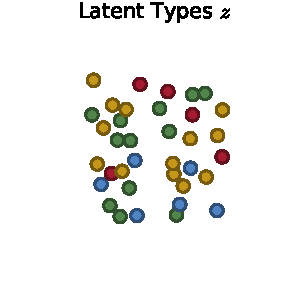
\includegraphics[width=\textwidth]{clustered_neurons}
%     \caption{}
%     \label{fig:fig1_z}
%   \end{subfigure}
%   \begin{subfigure}[b]{.3\textwidth}
%     \centering
%     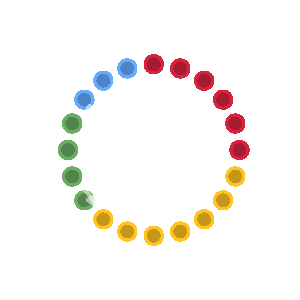
\includegraphics[width=\textwidth]{clustered_network}
%     \caption{}
%     \label{fig:fig1_W}
%   \end{subfigure}
%   \begin{subfigure}[b]{.3\textwidth}
%     \centering
%     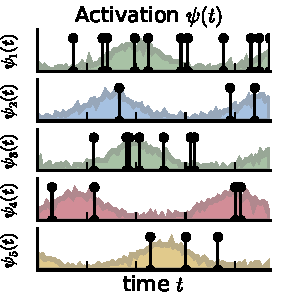
\includegraphics[width=\textwidth]{clustered_rates}
%     \caption{}
%     \label{fig:fig1_psi}
%   \end{subfigure}
%   \caption{Illustrative example of a generative model relating latent
%     structure to multineuronal spike trains via a functional
%     network. (a) Here, neurons have a latent class (\textit{red},
%     \textit{blue}, \textit{yellow}, or \textit{green}). 
%     (b) These classes govern the probability of functional
%     interactions for each pair of neurons. (c) The network
%     parameterizes an autoregressive model for the activation of the
%     neurons, which, in this example, give rise to the stochastic spike
%     trains we observe.}
% \label{fig:fig1}
% \end{figure}


\begin{figure}[t]
  \centering
  \begin{subfigure}[b]{\textwidth}
    \centering
    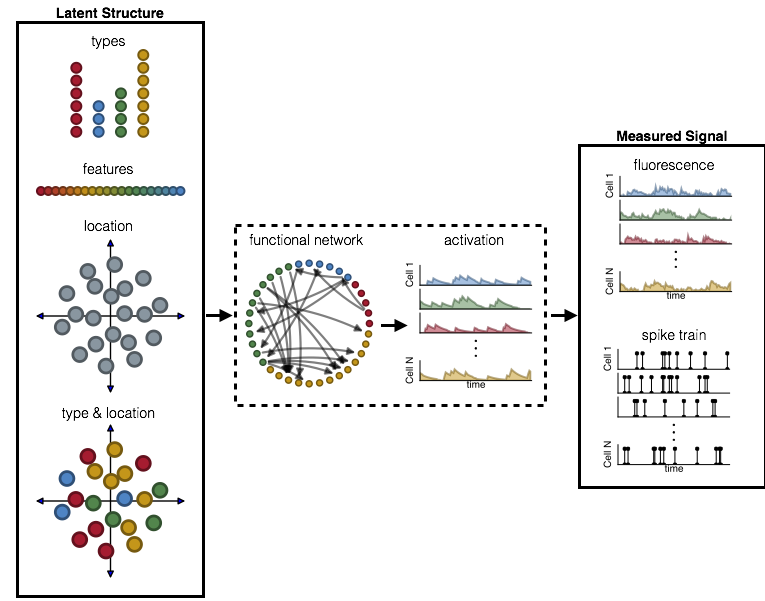
\includegraphics[width=\textwidth]{figures/ch3/figure1.png}
  \end{subfigure}
  \caption{Overview of model.}
  \label{fig:fig1}
\end{figure}

\section{Results}

\subsection{Synthetic Data}

\subsection{Retinal Ganglion Cells}

\subsection{Hippocampal Place Cells}

\subsection{Calcium Fluorescence}

\section{Methods}
Our primary contribution is a novel framework for discovering latent
network structure underlying neural activity.  This framework consists
of a probabilistic model relating structure to observed signals, an
efficient Bayesian inference algorithm capable of fitting this model,
and a model selection algorithm that enables principled comparison of
structural forms.

\subsection{Probabilistic Model}
A probabilistic model specifies a joint probability distribution over
measured signals, the underlying network, and latent structural
variables we wish to infer.  In our model, the measured signal from
neuron~$n$ in the~$t$-th time bin is denoted~$s_{t,n}$, which may 
denote either a discrete spike count or a real-valued signal, like 
the calcium fluorescence. In either case, this signal is assumed 
to be stochastically drawn from a distribution parameterized by 
an underlying, real-valued \emph{activation},~$\psi_{t,n}$,
and a static parameter,~$\nu_n$. The
activation is typically related to the expected spike count via
a logistic transformation,~$\sigma(\psi) = e^\psi \, (1+e^\psi)^{-1}$,
which has the property~$\sigma(-\psi) = 1-\sigma(\psi)$.

\begin{table}
\begin{center}
\begin{tabular}{c|c|c|c|c}
  \textbf{Distribution} & $p(s \given \psi, \nu)$ & Standard Form & $\bbE[s]$ & $\Var(s)$ \\
  \hline
  Gaussian & $\frac{1}{\sqrt{2 \pi \nu}}\exp \left \{ -\frac{1}{2 \nu} (s - \psi)^2 \right \}$
  & --- 
  & $\psi$ & $\nu$ \\
  Bernoulli & $\sigma(\psi)^s \, \sigma(-\psi)^{1-s}$
  & $\frac{(e^\psi)^s}{1+e^\psi}$
  & $\sigma(\psi)$ & $\sigma(\psi) \, \sigma(-\psi)$ \\
  Binomial & ${\nu \choose s} \, \sigma(\psi)^s \, \sigma(-\psi)^{\nu-s}$
  & ${\nu \choose s} \,\frac{(e^\psi)^s}{(1+e^\psi)^\nu}$
  & $\nu \sigma(\psi)$ & $\nu \sigma(\psi) \, \sigma(-\psi)$ \\
  Neg. Binomial & ${\nu + s -1 \choose s} \, \sigma(\psi)^s \, \sigma(-\psi)^{\nu}$
  & ${\nu +s - 1 \choose s} \,\frac{(e^\psi)^s}{(1+e^\psi)^{\nu+s}}$
  & $\nu e^\psi$ & $\nu e^\psi / \sigma(-\psi)$ \\
\end{tabular}
\end{center}
\caption{List of observation distributions.}
\label{tab:obs_models}
\end{table}

We consider the four observation models shown in Table~\ref{tab:obs_models}.
The Gaussian model assumes~$s_{t,n}$ is real-valued, and may be
appropriate for modeling calcium fluorescence, for example.
The Bernoulli distribution is appropriate for binary spike counts,
whereas the binomial and negative binomial have support
for~$s\in[0,\nu]$ and~$s \in [0, \infty)$, respectively.
Notably lacking from this list is the Poisson distribution,
which does not seem to be amenable to the augmentation schemes
we will derive below. Nevertheless, both the binomial and negative
binomial distributions converge to the Poisson under certain
limits, and they afford the added flexibility of modeling under- and
over-dispersed spike counts. Specifically, while the Poisson has unit 
dispersion (its mean is equal to its variance), the binomial distribution 
is always under-dispersed, since its mean always exceeds its variance, 
and the negative binomial is always over-dispersed, with variance greater 
than its mean.

The generalized linear model (GLM) \cite{Paninski-2004, Truccolo-2003, Pillow-2008} 
models the activation at time~$t$ as a weighted function of 
the spike counts at preceding times~${[0,t-1]}$. Specifically,
let,
\begin{align}
  \label{eq:glm_activation}
  \psi_{t,n} &\triangleq w_n^{(0)}  +                 
               \sum_{m=0}^N  \sum_{k=1}^K a_{n \from m} \, w_{n \from m}^{(k)}
               \left( \sum_{\Delta t=1}^{\Delta t_{\mathsf{max}}} \phi_{k, \Delta t} \cdot s_{t-\Delta t, m} \right) \\
             &= w_n^{(0)}  + \sum_{m=0}^N \sum_{k=1}^K a_{n \from m} \, w_{n \from m}^{(k)} \, \widehat{s}_{t,m}^{(k)} \\
  \label{eq:linear_activation}
             &= (\ba_{n} \odot \bw_n)^\trans \, \widehat{\bs}_t,
\end{align}
where~$w_n^{(0)}$ is the baseline activation of neuron~$n$,
$\bphi_{k,1:\Delta t_{\mathsf{max}}}$ is a basis function 
that weights the previous spike counts for 
offsets~${\Delta t \in [1, \Delta t_{\mathsf{max}}]}$
, the binary variable~${a_{n \from m} \in \{0,1\}}$ 
indicates whether or not there exists 
a directed connection from neuron~$m$ to neuron~$n$,
and~$w_{n \from m}^{(k)}$ captures the influence that
spikes on neuron~$m$ exert on neuron~$n$ at
offsets weighted by the~$k$-th basis function.  
Since the basis function and the signal 
are assumed to be fixed,  can precompute the inner sum, which is simply the 
convolution of the signal with the basis function, to get~$\widehat{s}_{t,m}^{(k)}$.
Since this is a linear function, we can combine the
connections, weights, and filtered spike trains into
vectors to get the linear form  in Eq.~\ref{eq:linear_activation}.
Here, we have,
\begin{align}
  \ba_n &=
    \bigg[
      1,  
      &a_{n \from 1}, & & \ldots, & & a_{n \from 1}, 
      & & \ldots, &
      &a_{n \from N}, & & \ldots, & &a_{n \from N} 
    &\bigg]^\trans, \\
  \bw_n &=
    \bigg[
      w_n^{(0)}, 
      &w_{n \from 1}^{(1)}, & & \ldots, & &w_{n \from 1}^{(K)}, 
      & &\ldots, &
      &w_{n \from N}^{(1)}, & & \ldots, & &w_{n \from N}^{(K)} 
      &\bigg]^\trans, \\
  \widehat{\bs}_t &=
    \bigg[
      1, 
      &\widehat{s}_{t,1}^{(1)}, & & \ldots, & &\widehat{s}_{t,1}^{(K)}, 
      & &\ldots, &
      &\widehat{s}_{t,N}^{(1)}, & & \ldots, & &\widehat{s}_{t,N}^{(K)} 
    &\bigg]^\trans,
\end{align}
and~$\odot$ dentoes the elementwise product. For convenience, we
let~$\bA$ and~$\bW$ refer to the~$N \times NK+1$ matrices obtained
by stacking the vectors~$\ba_n^\trans$ and~$\bw_n^\trans$, and we
let~$\widehat{\bS}$ denote the~$T \times NK+1$ matrix with rows
given by~$\widehat{\bs}_t^\trans$. The major difference between this formulation and that of the standard 
GLM is that here we have explicitly modeled the sparsity of the 
weights via the ``adjacency matrix'' $\bA$. Under the standard 
formulation, all weights are present, that is,~${a_{n \from m} \equiv 1}$.

Figure~\TODO{} illustrates the GLM dynamics. In this case, there is
one basis function ($K=1$) defined
by,~${\phi_{1,\Delta t} = e^{-\Delta t/\tau}}$.
Then~$\widehat{s}_{t,m,1}$ is a weighted sum of spikes in the
window~$[t-\Delta t_{\mathsf{max}},t-1]$, where the weights decay
according to an exponential function with time constant~$\tau$.  
If~${A_{n \from m}=1}$, indicating a
connection from neuron~$m$ to neuron~$n$, and
the weight,~$W_{n \from m,1}$, is positive, the influence will be
excitatory. If it is negative, the effect will be inhibitory.
Together, the weights~$\bW$ define a functional \emph{network} of
interactions.

The popularity of generalized linear models is due, in large part, to
the intuitive appeal of networks as a description of neuronal
dynamics.  While the weights of the GLM may not necessarily correspond
to direct synaptic connections, they provide an interpretable
representation of firing rate dynamics in terms of a functional
network. However, this interpretability is hampered by the fact that
there are~$O(N^2)$ weights to reason about, and as the number of
neurons,~$N$, grows, it becomes impossible to make sense of the entire
network.

We extend our probabilistic model with hierarchical latent variable
models that capture intuitive structure in the network, while
retaining the interpretable network-based representation that makes
the GLM so popular. We assume that each neuron is endowed with a set
of latent features that govern the probability of functional
interactions. Specifically, we consider two types of features:
discrete classes,~$c_n \in \{1, \ldots, C\}$, and continuous
locations,~$\bell_n \in \reals^D$. These can determine either the
probability of connection,~$\rho_{n \from m}$, or the mean and
variance of a multivariate Gaussian prior on the
weights,~$\bmu_{n \from m}$ and~$\bSigma_{n \from m}$.
Conditioned upon these latent variables, the connections and 
their weights are all conditionally independent of one another.
That is,
\begin{align}
  p(\ba_n, \bw_n \given c_n, \bell_n, \theta) = 
  p(\ba_n \given c_n, \bell_n, \theta) \, p(\bw_n \given c_n, \bell_n, \theta),
\end{align}
where
\begin{align}
  p(\ba_n \given c_n, \bell_n, \theta) 
  &= \prod_{m=1}^N \distBernoulli(a_{n \from m} \given \rho_{n \from m}), \\
  p(\bw_n \given c_n, \bell_n, \theta) 
  &= \distNormal(w_n^{(0)} \given \mu_0, \sigma^2_0 ) \prod_{m=1}^N 
     \distNormal(\bw_{n \from m} \given \bmu_{n \from m}, \, \bSigma_{n \from m}), \\
  &= \distNormal(\bw_n \given \bmu_n, \bSigma_n).
\end{align}
Here, we have combined the Gaussian factors into single multivariate Gaussian prior
with parameters,
\begin{align}
  \bmu_n 
    &= \begin{bmatrix}
      \mu_0 \\
      \bmu_{n \from 1} \\
      \vdots \\
      \bmu_{n \from N}
    \end{bmatrix}, & \text{ and } & &
  \bSigma_n 
  &= \begin{bmatrix}
    \sigma_0^2 &                     &        & \\
               & \bSigma_{n \from 1} &        & \\
               &                     & \ddots & \\
               &                     &        & \bSigma_{n \from N} 
    \end{bmatrix}.
\end{align}
As previously mentioned, the parameters~$\rho_{n \from m}$,~$\bmu_{n \from m}$, and~$\bSigma_{n \from m}$ 
may depend on~$c_n$,~$\bell_n$, and the parameters of the model,~$\theta$.
The form of these dependencies is a function of the underlying models, 
which we describe next.

\begin{table}
\begin{center}
\begin{tabular}{c|c|c}
Name & Latent Variable & $p(A_{n \from m≈})$ \\
\hline
Dense Model & --- & $1$ \\
Bernoulli Model & --- & $\rho$ \\
Stochastic Block Model & $c_n$ & $\rho_{c_n \from c_m}$ \\
Latent Distance Model & $\bell_n$ & $\sigma(-||\ell_n - \ell_m||_2^2 + \gamma_0)$
\end{tabular}
\end{center}
\caption{Binary Adjacency Matrix Models}
\label{tab:A_models}
\end{table}

Table~\ref{tab:A_models} defines the four adjacency models considered 
herein. The dense model corresponds to the standard GLM in which all
connections are present. The Bernoulli model is a spike-and-slab model 
in which each connection is an independent and identically distributed 
Bernoulli random variable with probability~$\rho$. This is also known 
as an Erd\"os-R\'enyi model. In the stochastic block model (SBM) 
\cite{Nowicki-2001}, the probability of connection depends on the class 
of the up and downstream neurons. The class assignments are drawn from
a categorical prior,~${c_n \sim \distCategorical(\bpi)}$, and the class
weights are given a conjugate, symmetric 
Dirichlet prior,~${\bpi \sim \distDirichlet(\alpha \bone_C)}$. The 
connection probabilities are given a conjugate beta 
prior,~${\beta_{c \from c'} \sim \distBeta(\alpha, \beta)}$. 
The latent distance model \cite{Hoff-2008} encodes the belief that 
connection probability should decrease with distance between latent 
locations. The locations are given spherical Gaussian 
priors,~$\bell_n \sim \distNormal(0, \eta \bI)$, and the scale is
drawn from an inverse gamma prior,~$\eta \sim \distInvGamma(1,1)$. The 
offset is given a standard normal prior,~$\gamma_0 \sim \distNormal(0, 1)$.


\begin{table}
\begin{center}
\begin{tabular}{c|c|c|c}
Name & Latent Variable & $\bmu_{n \from m}$ & $\bSigma_{n \from m}$\\
\hline
Gaussian Model & --- & $\bmu$ & $\bSigma$ \\
Stochastic Block Model & $c_n$ & $\bmu_{c_n \from c_m}$ & $\bSigma_{c_n \from c_m}$ \\
Latent Distance Model (${K=1}$) & $\bell_n$ & $-||\bell_n - \bell_m||_2^2 + \mu_0$ & $\sigma^2$
\end{tabular}
\end{center}
\caption{Gaussian Weight Models}
\label{tab:W_models}
\end{table}

Table~\ref{tab:W_models} defines the three weight models we
consider.  Each model defines the mean and variance of a multivariate
normal distribution,~$\bw_{n \from m} \sim \distNormal(\bmu_{n \from
  m}, \bSigma_{n \from m})$.  In the Gaussian model, all weights are
independent and identically distributed.  The stochastic block model,
has parameters for each pair of classes, each drawn from a normal
inverse-Wishart prior,~$(\bmu_{c \from c'}, \bSigma_{c \from c'}) \sim
\distNormalInvWishart(\mu_0, \kappa_0, \Sigma_0, \nu_0)$. Finally, we
consider a latent distance model, but only for the case where the
weights are scalar, i.e.~$K=1$. In this case, the distance between
points is inversely proportional to the mean weight.  For higher order
weights, additional assumptions would be required in order to relate
distance to vector weights. In this model, we assume standard normal
priors on the parameters~$\bell_n$ and~$\mu_0$.  The variance is given
an inverse gamma prior,~$\sigma^2 \sim \distInvGamma(\alpha, \beta)$.

Of course, many other models could be added to this list, and in the
discussion we will consider various extensions. An attractive feature
of this approach is that we may indeed draw on an extensive literature
of network models. For the purposes of this paper, we restrict our
attention to these models, based on latent classes and locations,
which are particularly interpretable and easily visualized.

We can now write down the joint probability of our probabilistic model.
Let~$\theta$ denote the parameters of the network model, like the connection
probabilities under the Bernoulli model or the class-specific mean and variance
under a stochastic block model for the weights. 
The joint probability is,
\begin{multline}
p(\bs, \{\nu_n, \ba_n, \bw_n, c_n, \bell_n\}_{n=1}^N, \theta) 
=  \\
p(\theta) \,
\prod_{n=1}^N \bigg[ \overbrace{p(c_n, \bell_n \given \theta)}^\text{latent variables} \, 
\overbrace{p(\ba_n, \bw_n \given \{c_m, \bell_m\}_{m=1}^N, \theta)}^\text{network} \, \\
\times \underbrace{ p(\nu_n) \prod_{t=1}^T  p \left(s_{t,n} \given \widehat{\bs}_{t}, \ba_n, \bw_n, \nu_n \right) }_\text{observation} \bigg].
\end{multline}
The joint probability
factorizes into the product of three pieces: the latent variables, the network, and the observed spikes and their corresponding observation parameters. Next, we will describe
how to perform efficient Bayesian inference of the latent variables
and the network, given the observed spike train and this probabilistic model.

\subsection{Bayesian Inference}
Inference is the process of evaluating the posterior distribution over latent variables given the observed signal, which is related to the joint distribution by Bayes' rule:
\begin{align}
p(\{\nu_n, \ba_n, \bw_n, c_n, \bell_n\}_{n=1}^N, \theta \given \bs)  
  &= \frac{p(\bs, \{\nu_n, \ba_n, \bw_n, c_n, \bell_n\}_{n=1}^N, \theta) }{p(\bs)}.
\end{align}
The denominator on the right hand side is known as the \emph{marginal likelihood} of the spike train. 
%It will play a crucial role in model selection. 

It is computationally intractable to compute this posterior exactly and it has no simple closed form solution, so we must instead resort to approximate methods. 
We use Markov chain Monte Carlo (MCMC) methods to collect samples from this posterior distribution.
With these samples, we can compute unbiased expectations with respect to the posterior distribution.
For example, we can compute the expected probability that two neurons belong to the same class, the expected weight of a functional connection between two neurons, or the expected predictive likelihood of heldout test data.


\subsubsection{Collapsed network updates}
The most challenging aspect of inference is sampling the
posterior distribution over connections,~$\bA$. In the
dense model, where~$a_{n \from m} \equiv 1$, the posterior
distribution over weights is often log concave, which
makes it easy to find the MAP estimate and characterize
the local uncertainty around the most likely weights.
When the connectivity matrix is sparse, there are instead
many modes corresponding to different patterns of
connectivity. While this makes inference more challenging,
sparse connectivity is an important feature that
contributes to the interpretability of the model.

Fortunately, we can make posterior inference of the
network considerably more efficient by integrating over
possible weights and sampling the binary adjacency
matrix from its marginal distribution. 
First, consider the Gaussian observation model.
Since~$\psi_{t,n}$ is linear in~$\bw_n$, the likelihood
is conjugate with the Gaussian prior, and hence the
posterior is Gaussian as well. We can
compute the posterior distribution in closed form:
\begin{align}
  p(\bw_n \given \widehat{\bS}, \ba_n, \bmu_n, \bSigma_n)
  &\propto
  \distNormal(\bw_n \given \bmu_n, \bSigma_n) \,
  \prod_{t=1}^T \distNormal(s_{t,n} \given (\ba_n \odot \bw_n)^\trans \, \widehat{\bs}_t, \, \nu_n) \\
  &= \distNormal(\bw_n \given \bmu_n, \bSigma_n) \,
  \distNormal(\bs_n \given (\ba_n \odot \bw_n)^\trans \, \widehat{\bS}, \, \nu_n \bI) \\
  \label{eq:w_conditional}
  &\propto \distNormal(\bw_n \given \widetilde{\bmu}_n, \widetilde{\bSigma}_n),
\end{align}
where
\begin{align}
  \widetilde{\bSigma}_n &= \left[ \bSigma_n^{-1} +
  \left(\widehat{\bS}^\trans (\nu_n^{-1} \bI) \widehat{\bS} \right) \odot (\ba_n \ba_n^\trans) \right]^{-1}, \\
  \widetilde{\bmu}_n &= \widetilde{\bSigma}_n \left[ \bSigma_n^{-1} \bmu_n +
  \left(\widehat{\bS}^\trans (\nu_n^{-1} \bI)\bs_n \right) \odot \ba_n \right].
\end{align}

Given this closed-form Gaussian conditional, we can also compute
the conditional distribution over just~$\ba_n$, integrating out
the corresponding weights,~$\bw_n$:
\begin{align}
  p(\ba_n \given \widehat{\bS}, \brho_n, \bmu_n, \bSigma_n)
  &= \int p(\ba_n, \bw_n \given \widehat{\bS}, \brho_n, \bmu_n, \bSigma_n) \, \mathrm{d} \bw_n \\
  &\propto p(\ba_n \given \brho_n) \, \int p(\bw_n \given \widehat{\bS}, \ba_n, \bmu_n, \bSigma_n) \, \mathrm{d} \bw_n \\
  \label{eq:a_conditional}
  &= p(\ba_n \given \brho_n) \, \frac{\big| \bSigma_n \big|^{-\frac{1}{2}} \exp \Big \{-\frac{1}{2} \bmu_n^\trans \bSigma_n^{-1} \bmu_n \Big \} }
  {\big| \widetilde{\bSigma}_n \big|^{-\frac{1}{2}} \exp \Big \{-\frac{1}{2} \widetilde{\bmu}_n^\trans \widetilde{\bSigma}_n^{-1} \widetilde{\bmu}_n \Big \}}.
\end{align}
Thus, we can efficiently sample from the conditional
distribution of~$\ba_n$ and~$\bw_n$ by first iterating
over each neuron~${m \in \{1, \ldots, N\}}$ and sampling
a new value of~$a_{n \from m}$, fixing the values of~$a_{n \from m'}$
for~$m' \neq m$ and integrating out the value of~$\bw_n$.
To do so, we simply evaluate the marginal probability in Eq.~\ref{eq:a_conditional}
for both values of~$a_{n \from m}$ and resample accordingly.
This is a valid Gibbs step. Once~$\ba_n$ has been completely
resampled, we can sample a new value of~$\bw_n$ from its multivariate
Gaussian conditional distribution, given by~Eq.~\ref{eq:w_conditional}.

\subsubsection{\polyagamma augmentation for discrete observations}
When the observations are not Gaussian, the conditional distribution
of~$\bw_n$ cannot be computed in closed form and the collapsed
updates are intractable. To circumvent this problem, we leverage
recently developed augmentation schemes for Gaussian models with
discrete observations \cite{polson2013bayesian, Pillow2012}. The
idea is to augment the observations,~$s_{t,n}$, with auxiliary
variables,~$\omega_{t,n}$, such that conditioned upon the
auxiliary variables, the discrete likelihood appears Gaussian.

First, notice that the discrete likelihoods in Table~\ref{tab:obs_models}
can all be put into  a ``standard'' form in which the probability
mass function can be written,
\begin{align}
  p(s \given \psi, \nu) &= c(s, \nu) \, \frac{(e^\psi)^{a(s, \nu)}}{(1+e^\psi)^{b(s, \nu)}},
\end{align}
for some functions,~$a$,~$b$, and~$c$ that do not depend on~$\psi$.
The integral identity at the heart of the P\'{o}lya-gamma augmentation scheme  is
\begin{align}
\label{eq:pg_identity}
\frac{(e^{\psi})^a}{(1+e^{\psi})^b} = 2^{-b} e^{\kappa \psi} \int_{0}^{\infty} e^{-\omega \psi^2 /2} \, p_{\mathrm{PG}}(\omega \given b, 0) \, \mathrm{d}\omega,
\end{align}
where~${\kappa=a-b/2}$ and~$p(\omega\given b, 0)$ is the density of the P\'{o}lya-gamma
distribution~${\distPolyaGamma(b, 0)}$, which does not depend on $\psi$.

Using Eq.~\ref{eq:pg_identity} along with priors~$p(\psi)$ and~$p(\nu)$, we can write the joint density of $(\psi, s, \nu)$ as
\begin{align}
  \label{eq:pg_joint}
  p(s, \nu, \psi)
  &= p(\nu) \, p(\psi) \, c(s, \nu) \frac{(e^\psi)^{a(s, \nu)}}{(1+e^\psi)^{b(s, \nu)}} \\
  &= \int_0^\infty
  p(\nu) \, p(\psi) \, c(s, \nu) \, 2^{-b(s, \nu)} e^{\kappa(s, \nu) \psi} e^{-\omega \psi^2/2} \, p_{\mathrm{PG}}(\omega \given b(s, \nu), 0) \; \mathrm{d}\omega.
\end{align}
The integrand of Eq.~\ref{eq:pg_joint} defines a joint density on $(s, \nu, \psi, \omega)$ which admits $p(s, \nu, \psi)$ as a marginal density.
Conditioned on these auxiliary variables $\omega$, we have that the likelihood as a function of~$\psi$ is,
\begin{align}
  p(s \given \psi, \nu, \omega)
  &\propto e^{\kappa(s, \nu) \psi} e^{- \omega \psi^2/2} 
\propto \distNormal \left(\frac{\kappa(s, \nu)}{\omega} \, \bigg| \, \psi, \, \frac{1}{\omega} \right).
\end{align}

Thus, we effectively have a Gaussian likelihood for~$\psi$, after conditioning 
on~$s$ and~$\omega$. Now we can apply this augmentation scheme to the full
model, introducing auxiliary variables,~$\omega_{t,n}$ for each spike count,~$s_{t,n}$.
Given these variables, the conditional distribution of~$\bw_n$ can be computed in closed form,
as before. Let,
\begin{align}
  \bkappa_n
  &= \begin{bmatrix} \kappa(s_{1,n}, \nu_n), &\ldots, &\kappa(s_{T,n}, \nu_n)
  \end{bmatrix}^\trans,
\end{align}
and
\begin{align}
  \bOmega_n &= \diag \left(
  \begin{bmatrix}
    \omega_{1,n}, & \ldots, & \omega_{T,n}
  \end{bmatrix}
  \right).
\end{align}
Then we have~$
  p(\bw_n \given \bs_n,  \widehat{\bS}, \ba_n, \bmu_n, \bSigma_n, \bomega_n, \nu_n)
  \propto \distNormal(\bw_n \given \widetilde{\bmu}_n, \widetilde{\bSigma}_n)$,
where
\begin{align}
  \widetilde{\bSigma}_n &= \left[ \bSigma_n^{-1} +
  \left(\widehat{\bS}^\trans \bOmega_n \widehat{\bS} \right) \odot (\ba_n \ba_n^\trans) \right]^{-1}, \\
  \widetilde{\bmu}_n &= \widetilde{\bSigma}_n \left[ \bSigma_n^{-1} \bmu_n +
  \left(\widehat{\bS}^\trans \bkappa_n \right) \odot \ba_n \right].
\end{align}

Having introduced auxiliary variables, we must now also derive
Markov transitions to update them as well. Fortunately, the
\polyagamma distribution is designed such that the conditional
distribution of the auxiliary variables is just a ``tilted'' \polyagamma
distribution,
\begin{align}
  p(\omega_{t,n} \given s_{t,n}, \nu_n, \psi_{t,n})
  &= p_{\mathrm{PG}}(\omega_{t,n} \given b(s_{t,n}, \nu_n), \, \psi_{t,n}).
\end{align}
These auxiliary variables are conditionally independent and hence can
be updated in parallel. Moreover, efficient algorithms are available
to generate \polyagamma random variates~\cite{windle2014sampling}, and
we have ported these to Python\footnote{\url{https://github.com/slinderman/pypolyagamma}}.

\subsubsection{Updating latent variables and parameters}
Given the network and the spike train, the conditional distributions 
for the latent variables,~$\{c_n, \bell_n\}$, and the parameters,~$\theta$ and~$\{\nu_n\}$,
are easy by design. 

\begin{itemize}
  \item \textit{Latent class updates}:
    If a stochastic block model is used for either the adjacency matrix
    or the weights, then it is necessary to sample the class assignments
    from their conditional distribution. We iterate over each neuron and
    update its assignment given the rest by sampling from the conditional
    distribution. For example, if~$c_n$ governs a stochastic block model
    for the adjacency matrix, the conditional distribution of the label
    for neuron~$n$ is given by,
    \begin{align}
      p(c_n = c \given \bc_{\neg n}, \bA, \theta)
      &\propto \pi_{c} \,
      \prod_{m=1}^N p(a_{n \from m} \given \rho_{c \from c_m}) \,
                    p(a_{m \from n} \given \rho_{c_m \from c}),
    \end{align}
    where~$\theta = \{\bpi, \{\rho_{c \from c'}\} \}$. For stochastic block
    models of the weight matrix,~$\bW$, the conditional distribution
    depends on~$\bw_{n \from m}$ and~$\bw_{m \from n}$ instead.

    Given the class assignments and the network, the
    parameters~$\rho_{c \from c'}$,~$\bmu_{c \from c'}$,~$\bSigma_{c \from c'}$, and~$\bpi$ are easily updating
    according to their conditional distributions, since the model is
    conjugate.
    
  \item \textit{Latent location updates}:
    We resample the locations using hybrid Monte Carlo (HMC) \cite{Neal10}.
    Since the latent variables are continuous and unconstrained,
    this method is quite effective.

    In addition to the locations, the latent distance model is parameterized
    by a location scale,~$\eta$. Given the locations and an inverse gamma
    prior, the inverse gamma conditional distribution can be computed in
    closed form.
    
    The remaining parameters include the log-odds,~$\gamma_0$, if the
    distance model applies to the adjacency matrix. This can be
    sampled alongside the locations with HMC.  For a latent distance
    model of weights, the baseline mean and
    variance,~$(\mu_0,\sigma^2)$, are conjugate with a normal
    inverse-gamma prior.
    
  \item \textit{Observation parameter updates}:
    The observation parameter updates depend on the particular distribution.
    For Gaussian observations,~$\nu_n$ is the observation variance, and
    it is conjugate with an inverse gamma prior.
    Bernoulli observations have no parameters.
    In the binomial model,~$\nu_n$ corresponds to the maximum number of
    possible spikes --- this is best set a priori.
    For negative binomial spike counts, the shape parameter~$\nu_n$ can
    be resampled as in~\cite{Zhou2012}.

    
\end{itemize}

\subsection{Model Selection}
We have constructed a probabilistic model that supports a variety
of network models, including the four adjacency models and the three
weight models described above. How can we compare these models in
a principled manner? We argue that the typical approach of measuring
predictive log likelihood on held-out time bins is insufficient, since
it relies only on having accurately estimated the network,~$\bA$ and~$\bW$.
It doesn't matter how likely that network is under the latent variable
model, predictive likelihood on held-out time bins only measures the
quality of the network at making predictions. Instead, we advocate
for an alternative measure based on predicting the activity of held-out
neurons. To perform well on this task, we must first learn an accurate
model for the structure underlying the network so that we can
sample latent variables for the new neuron, which in turn allow us to
sample a weighted set of functional connections for that neuron and
finally compute the predictive log likelihood.

The objective we measure is the probability of a new spike
train~$\bs_{n^*}=[s_{1,n^*}, \ldots, s_{T,n^*}]$, given the
observed spike train. To compute this, we must integrate
over the latent variables and parameters underlying the
observed spike train, as well as those underlying the
new spike train. 
Let~$\bZ = \{\{\bw_n, \ba_n, \nu_n, c_n, \bell_n\}_{n=1}^N, \theta\}$, and
let~$\bz_{n^*} = \{\nu_{n^*}, \bw_{n^*}, \ba_{n^*}, c_{n^*}, \bell_{n^*}\}$.
This objective can be written,
\begin{align}
  p(\bs_{n^*} \given \bS) &\approx
  \int p(\bs_{n^*} \given \bz_{n^*}, \bS) \, p(\bz_{n^*} \given \bZ) \, p(\bZ \given \bS) \,
  \mathrm{d} \bz_{n^*} \, \mathrm{d} \bZ \\
  &\approx
  \frac{1}{Q} \sum_{q=1}^Q p(\bs_{n^*} \given \bz_{n^*}^{(q)}, \bS),
  %\int p(\bs_{n^*} \given \bS, \bz_{n^*}) \,
  %p(\bz_{n^*} \given \{c_n, \bell_n\}, \theta) \, \mathrm{d}\bz_{n^*}
\end{align}
where
\begin{align}
  \bz_{n^*}^{(q)} &\sim p(\bz_{n^*} \given \bZ^{(q)}),
  &\text{ and }& & 
  \bZ^{(q)} &\sim p(\bZ \given \bS).
\end{align}
The samples~$\{\bZ^{(q)}\}_{q=1}^Q$ are the posterior samples generated
by the MCMC algorithm presented above. For each sample, we
sample a new set of latent variables and connections for neuron~$n^*$,
given the parameters included in~$\bZ^{(q)}$. These, combined with
the spike train, enable us to compute the likelihood of~$\bs_{n^*}$.

This approach constitutes a minor approximation:
the new spike train and the original spike train are not
conditionally independent. It is possible that there are
significant connections from~$n^*$ to neurons in the training
population, and if we had known those connections, we would
have inferred different latent variables and parameters for
the training population. We assume that these effects are small,
i.e. we would find similar class assignments even without observing~$n^*$.
This is reasonable if we are only considering a single neuron~$n^*$
and the training population is reasonably large, say~$N \geq 20$.
In fact, this assumption is fundamental to the generalized
linear model. Without it, the inferred weights and predictions
would be highly sensitive to the addition of a single neuron.
In practice this is rarely the case.


\section{Discussion}

\subsection{Related Work}
\begin{itemize}
\item Simple clustering and dimensionality reduction of spike train matrices
\item Network models
\item Generalized linear models
\item Bayesian inference (go through Liam's work)
\item Polya-gamma augmentation
\end{itemize}
